\section{From a Model Graph to Runtime Assignments}
Local preparation verifies a reusable model package, its source identity, and supported interfaces. In this chapter, \texttt{PreparedModel} denotes that locally validated, reusable model package and session state; it is not a Provider assignment, resource reservation, or proof that a remote runner is ready.

After ACK collection closes, the native planner validates offers, enumerates supported partitions, and validates placement. A reusable or manually authored template may constrain that search; it does not preselect the runtime Providers.

The planner obtains artifact references and seals the execution plan before committing it through the NDNSF runtime. After authenticating Selection, each selected Provider obtains, assembles, or reuses its permitted resources before execution.

\begin{figure}[htbp]\singlespacing\centering
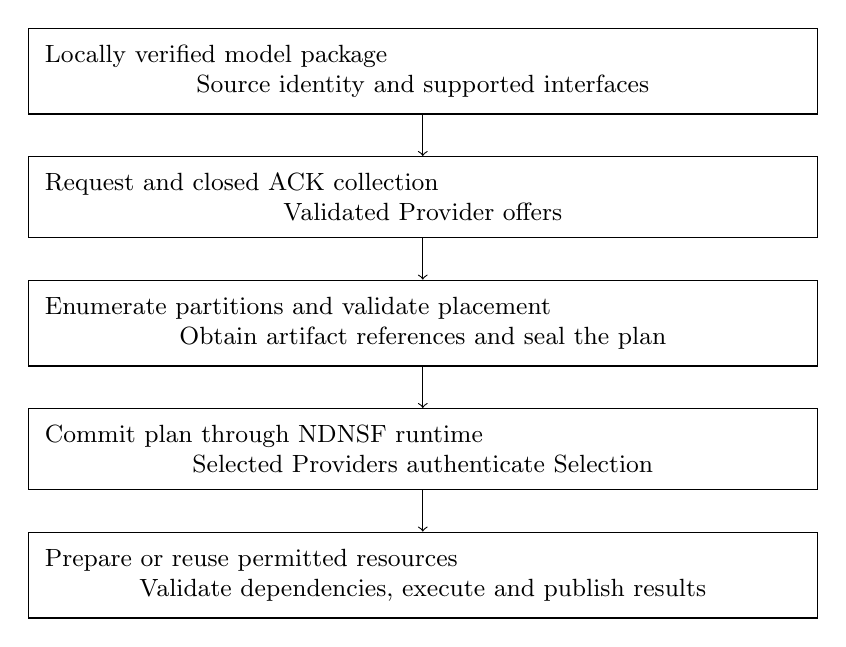
\begin{tikzpicture}[every node/.style={draw,align=center,font=\small,text width=9.6cm,inner sep=6pt}]
\node (model) at (0,0) {Locally verified model package\newline Source identity and supported interfaces};
\node (template) at (0,-1.6) {Request and closed ACK collection\newline Validated Provider offers};
\node (assign) at (0,-3.2) {Enumerate partitions and validate placement\newline Obtain artifact references and seal the plan};
\node (plan) at (0,-4.8) {Commit plan through NDNSF runtime\newline Selected Providers authenticate Selection};
\node (execute) at (0,-6.4) {Prepare or reuse permitted resources\newline Validate dependencies, execute and publish results};
\draw[->] (model)--(template);\draw[->] (template)--(assign);
\draw[->] (assign)--(plan);\draw[->] (plan)--(execute);
\end{tikzpicture}
\caption{Model preparation and request-specific planning in the native path. Arrows show processing order; model, device, and recovery coverage still require separate validation.}
\end{figure}

Each fragment contract needs defined input and output tensor names, shapes or supported dynamic-shape constraints, element types, serialization, and model-version compatibility. A split across a skip connection or a branching graph may have multiple live outputs, not a single vector. The receiving fragment must obtain all required inputs before execution. A useful negative test supplies a correctly signed tensor with the wrong shape or model identity: protocol provenance may be valid while the application contract is not.

Pipeline partitioning assigns consecutive computation stages and transfers their boundary tensors. Tensor parallelism splits an operation across participants and adds exchanges such as reductions or gathers. Model replication assigns independent work to complete copies. These are different execution strategies. Early exit changes how much model computation is performed~\cite{branchynet}; combining predictions from several models changes the analysis method. Both must be separated from placement effects. Edge--cloud describes device placement, not a distinct partition operator. ONNX export supplies a graph representation~\cite{onnx}; usable cuts and collective operations still depend on the supported runtime and model operators.

Preparation cost matters when a Provider lacks the required artifact or compatible loaded session. Evaluation should distinguish artifact transfer, session creation, accelerator memory allocation, and execution. A warm run that reuses resident weights cannot be compared to a cold baseline without reporting that difference. Placement can favor a Provider that already holds compatible state, but that policy must respect request authorization and cannot assume that cached state is transferable to any new request.

\section{Planning Inputs, Feasibility, and Policy Comparisons}
The planning study considers a bounded set of supported partition candidates. It separates feasibility constraints from optimization preferences: an unsupported operator, an incompatible tensor contract, or insufficient memory excludes an assignment; estimated execution or transfer time ranks otherwise feasible assignments. Estimates need a stated source and measurement age. A Provider's positive ACK is a willingness report, not an independently verified hardware benchmark.

\begin{table}[htbp]\centering\small
\caption{Inputs to the proposed DI planning comparison. These are evaluation dimensions, not a claim of a completed general optimizer.}
\begin{tabularx}{\textwidth}{p{.25\textwidth}XX}
\toprule Planning input & Feasibility / cost question & Experimental control\\\midrule
Model and partition contract & Operators, precision, tensor interfaces and compatible artifacts & Freeze model/export identity and supported cuts\\\midrule
Device resources & Weights, activations, workspace and retained key/value (K/V) state fit & Measure peak memory; do not use weight size alone\\\midrule
Computation and communication & Do capacity or execution-time benefits justify transfer costs? & Profile boundary bytes and per-stage time under the same load\\\midrule
Preparation and residency & Are artifacts, sessions and compatible state already present? & Separate cold preparation from warm execution\\\midrule
Permission and availability & Can each assigned role obtain its required objects before the deadline? & Apply authorization and deadline constraints before ranking\\\bottomrule
\end{tabularx}\end{table}

Compare a fixed valid mapping, a simple resource-aware mapping, and any implemented adaptive policy on the same Provider candidates and supported partitions. Record planning time, per-Provider utilization, and end-to-end cost. Where a policy predicts completion time, compare its prediction with the observed value; a policy using only feasibility rules needs no timing-prediction claim. If no complete feasible assignment exists, report that outcome rather than silently dropping a dependency. The initial question is whether runtime information improves assignment under stated conditions. Model splitting, Provider selection, and data-dependency enforcement remain independently testable.

\section{Tensor Exchange and Autoregressive State}
For a pipeline, an upstream fragment produces an activation tensor, makes it available as protected named Data, and supplies its reference through the declared dependency. The downstream fragment retrieves and validates that object, checks the tensor contract, and performs its assigned computation. A fan-out reuses an upstream output for several authorized consumers. A fan-in waits for the set of inputs required by the computation. The collaboration protocol decides which producers and edges are permitted; DI decides whether the tensor values and layouts are suitable for the model.

Autoregressive inference adds a dependency across decoding steps. When K/V caching is enabled, computation after prefill uses the preceding token and retained K/V state instead of recomputing the full prefix. With layer-based partitioning, each participating runtime can retain the K/V tensors for its assigned layers. A generated token or the information needed to select it returns to the component driving the next decoding step. Consequently, the forward path within one evaluation can follow a directed acyclic graph while the whole generation process repeatedly traverses that graph over time.

Keeping weights in accelerator memory does not eliminate the logical K/V inputs. A runtime may reuse device buffers and bind them directly rather than serialize and transmit the entire cache on each step~\cite{ortkvcache}. Reassignment or conversation continuation needs an explicit compatibility and state-transfer policy; silently starting a replacement with unrelated K/V state is not valid recovery. The evaluation separates savings from local K/V reuse, remote transfer costs, and framework orchestration costs.

The initial numerical validation should compare a supported partitioned execution with an unsplit execution of the same model, precision, inputs, and decoding policy. Appropriate tensor tolerances or deterministic output comparisons must be specified before measurement. A small synthetic model can validate a tensor route, but cannot establish memory feasibility, throughput, or recovery for a large pretrained model. These controls make it possible to distinguish a working communication path from a correct and useful distributed-inference application.

We are preparing multi-node GPU experiments on TigerCluster, the external multi-GPU cluster used for this evaluation, to evaluate NDNSF-DI. Providers will run on separate GPU nodes to check inference correctness and measure end-to-end latency, inter-Provider data-transfer overhead, and peak GPU memory use. These cluster experiments will complement, rather than replace, UAV wireless and mobility tests.
